\begin{problem}{Мишень}{стандартный ввод}{стандартный вывод}{1 секунда}{256 мегабайт}

В соревнованиях по стрельбе использовалось электронное оружие. Мишень состоит из 10 концентрических окружностей, радиусы окружностей уменьшаются с шагом в 2 единицы, центральная окружность имеет радиус 2 единицы.  Стрелок выполняет 10 выстрелов.

Помощник крепил мишени на табло неаккуратно, поэтому центр мишени оказывался смещенным относительно центра табло на число $N$ по оси $OX$, и на число $K$ по оси $OY$.

\begin{figure}[h]
\centering
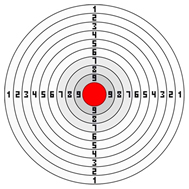
\includegraphics[width=.4\textwidth, bb=0 0 200 200]{Target.jpg}
\end{figure}

Напишите программу для подсчета очков стрелявших, если табло выдает декартовы координаты точки попадания относительно центра табло, а очки должны начисляться по мишени, как показано на рисунке. Если пуля попала в центр мишени, то начисляется 10 очков, а если на границу двух зон с разным количеством очков, то~--- большее значение. 



\InputFile
Входной файл содержит 11 строк, в каждой содержится по 2 вещественных числа. В первой строке~--- числа $N$ и $K$ ($-20 \le N, K \le 20$), записанные через пробел, в десяти следующих~--- по два вещественных числа в интервале от $-20$ до $20$.

\OutputFile
Выходной файл должен содержать одно целое число~--- количество очков, набранных стрелком. 

\Examples

\begin{example}
\exmpfile{example.01}{example.01.a}%
\end{example}

\begin{example}
    \exmpfile{example.02}{example.02.a}%
\end{example}

\end{problem}

